\let\negmedspace\undefined
\let\negthickspace\undefined
\documentclass[journal,12pt,onecolumn]{IEEEtran}
\usepackage{pgfplots}
\pgfplotsset{compat=1.17}
\usepackage{cite}
\usepackage{amsmath,amssymb,amsfonts,amsthm}
\usepackage{algorithmic}
\usepackage{graphicx}
\usepackage{textcomp}
\usepackage{xcolor}
\usepackage{txfonts}
\usepackage{listings}
\usepackage{enumitem}
\usepackage{mathtools}
\usepackage{gensymb}
\usepackage{comment}
\usepackage[breaklinks=true]{hyperref}
\usepackage{tkz-euclide} 
\usepackage{listings}
\usepackage{gvv}                                        
\def\inputGnumericTable{}                                 
\usepackage[latin1]{inputenc}                                
\usepackage{color}                                            
\usepackage{array}                                            
\usepackage{longtable}                                       
\usepackage{calc}                                             
\usepackage{multirow}                                         
\usepackage{hhline}                                           
\usepackage{ifthen}                                           
\usepackage{lscape}
\newtheorem{theorem}{Theorem}[section]
\newtheorem{problem}{Problem}
\newtheorem{proposition}{Proposition}[section]
\newtheorem{lemma}{Lemma}[section]
\newtheorem{corollary}[theorem]{Corollary}
\newtheorem{example}{Example}[section]
\newtheorem{definition}[problem]{Definition}
\newcommand{\BEQA}{\begin{eqnarray}}
\newcommand{\EEQA}{\end{eqnarray}}
\newcommand{\define}{\stackrel{\triangle}{=}}
\theoremstyle{remark}
\newtheorem{rem}{Remark}
\begin{document}
\bibliographystyle{IEEEtran}
\vspace{3cm}
\title{GATE GE 81Q}
\author{EE23BTECH11021 - GANNE GOPI CHANDU$^{*}$% <-this % stops a space
}
\maketitle
\bigskip
\renewcommand{\thefigure}{\theenumi}
\renewcommand{\thetable}{\theenumi}
\bibliographystyle{IEEEtran}
\textbf{Question}\\
The value of the convolution of $f(x) = 3\cos(2x)$ and $g(x) = \frac{1}{3}\sin(2x)$ where $x \in [0, 2\pi)$, at $x = \frac{\pi}{3}$, is (Rounded off to 2 decimal places)\\
\textbf{Solution}\\
The f(x) = $3\cos(2x)$ the  Fourier series is
\begin{align}
    f(x)&= a_0 + \sum_{n=1}^{\infty} a_n \cos(2nx)
\end{align}
where $b_n=0$ since  f(x)   is even function
\begin{align}
    a_0&= \frac{1}{\pi} \int_{0}^{2\pi} 3\cos(2x) dx = 0\\
    a_n&= \frac{1}{\pi} \int_{0}^{2\pi} 3\cos(2x) \cos(2nx) dx
\end{align}
 For $ g(x) = \frac{1}{3}\sin(2x) $ the Fourier series is:
 \begin{align}
     g(x)&= \sum_{n=1}^{\infty} b_n \sin(2nx)
 \end{align}
The $a_0=a_n=0$ since g(x) is a odd function
\begin{align}
   b_n&= \frac{1}{\pi} \int_{0}^{2\pi} \frac{1}{3}\sin(2x) \sin(2nx) dx 
\end{align}
Let's calculate the $ b_n $ coefficients for $ g(x) $:
\begin{align}
     b_n&= \frac{1}{\pi} \int_{0}^{2\pi} \frac{1}{3}\sin(2x) \sin(2nx) dx \\
     b_n&= \frac{1}{3\pi} \left[\frac{1}{2}\int_{0}^{2\pi} \left(\cos\left((2n-1)x\right) - \cos\left((2n+1)x\right)\right) dx\right]\\
     b_n&= \frac{1}{3\pi} \left[\frac{1}{2} \left(\left[\frac{\sin\left((n-1)2x\right)}{2(n-1)} - \frac{\sin\left((n+1)2x\right)}{2(n+1)}\right]_{0}^{2\pi}\right)\right] \\
     b_n&= \frac{1}{3\pi} \left[\frac{1}{2} \left(0 - 0 - 0 + 0\right)\right] = 0 
\end{align}
Since all $ b_n $ coefficients are zero
\begin{align}
    \brak{ f * g }(x)&= 0
\end{align}
So, the convolution of $f(x)$ and $g(x)$ at $x = \frac{\pi}{3}$ is $0$.
\begin{figure}
    \centering
    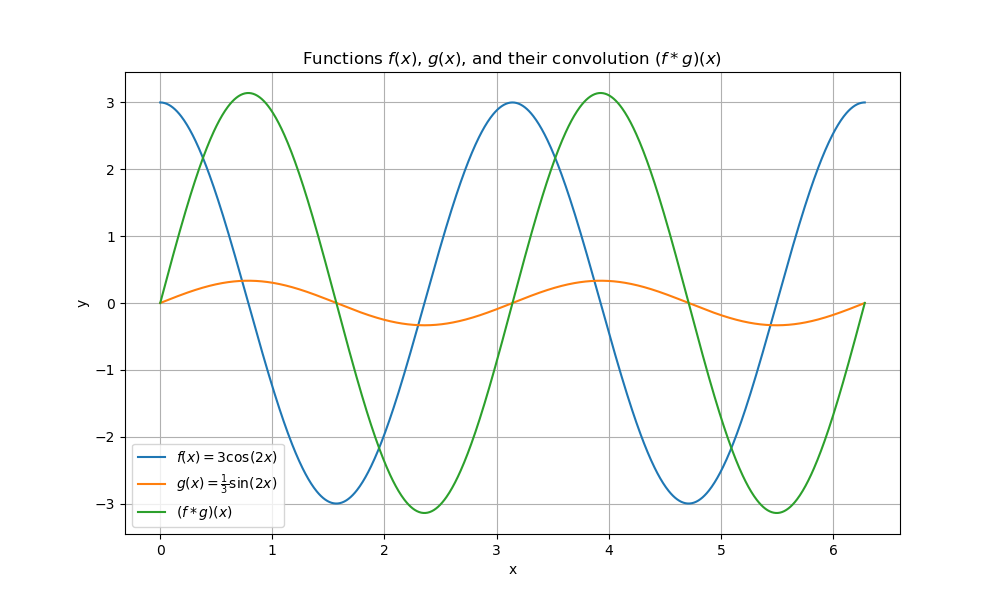
\includegraphics[width=1.0\linewidth]{Figure_3.png}
    \caption{Plot of y vs x}
    \label{fig:2}
\end{figure}
\end{document}
